\chapter{System Specification}
\label{cha:system}

\section{Overall User Experience}
The user experience of the system must be considered for two different use cases. The first is a user receiving a pre-build and pre-programmed sensor transducer in order to perform measurements. The second is a user adapting the system to incorporate the sensors needed for his use case and assembling the required hardware.

\subsection{Measurement Workflow}
A user equipped with a pre-build device should be able to trigger a measurement with a single button push. 

Before being able to start the first measurement it is acceptable if the following steps are necessary:
\begin{itemize}
\item Connecting a power source to the transducer
\item Pairing the hardware module in Android Bluetooth settings
\item Starting the application software
\item Choose the hardware module in the application settings
\item Enable the connection in the application settings
\end{itemize}

The transducer device should then be ready to send data to the application software after a hardware button is pressed.

\subsection{Adaption to Use Case}
Adapting the system to a use case requiring specific sensors should be possible by performing the following steps:

\begin{itemize}
\item Finding a sensor model that can be interfaced with Arduino
\item Designing the appropriate electronic circuit to connect the sensor to an Arduino
\item Building the circuit
\item Extend the existing software to support the connected sensor
\item Deploy and test the embedded software
\end{itemize}

There should be no need to modify the Android application software as it should be designed to support arbitrary sensor types as long as the transmission protocol is respected.

\subsection{User Interface}
Apart from the button triggering a measurement, the user interface is a mostly a part of the application software. The application software should include at least the following features:

\begin{itemize}
	\item Visualisation of the measurement data as a list
	\item Visualisation of the locations where measurements have been made
	\item Recording of geolocation data (to be used if there is no discrete hardware GPS module or the module has failed)
	\item Exporting the data in a .csv file appropriate for different target applications like Microsoft Excel and Matlab
\end{itemize}

\subsubsection{Design Considerations}
The design of the application software should be clear and simple to use. Android users should not be surprised by unexpected application behavior. Where possible, native design elements and user interface paradigms should be used.

\section{Transmission Technology Selection}
Android devices generally offer a multitude of communication technologies which might be suited for communications between the transducer device and the Android application software.

\paragraph{Cellular Networks}
Cellular networks provide internet connectivity, voice and text message service covering wide areas. The spectrum used for these networks is normally regulated and can only be used having an appropriate contract with a network provider. This leads to higher operation cost when using cellular networks for communication purposes. The main advantage of using cellular networks would be the independence from the smartphone as data can be transmitted to the smartphone over long distances and buffered by the network or an internet service. While in Europe cellular network coverage is almost ubiquitous, in other parts of the world coverage might be spotty and using cellular network technology would impose additional data buffering needs on the system.

\paragraph{IEEE 802.11 (WLAN/WiFi)}
Wireless Local Area Networks (WLAN) are widely used for internet connections and general networking over medium (around 10 meters) distance. Using WLAN technology for a mobile use case has the major disadvantage of a device being only able to connect to one network at a time. This would mean the transducer must be either connected to the network that is used by the Android device for other communications as well (which might not even be possible for networks using complex authentication schemes like \emph{eduroam}). When used in a region without a known WLAN available, one of the devices would need to establish a network and make the other join it. 

\paragraph{Bluetooth}
The Bluetooth technology is used for so-called personal area networks. Bluetooth was originally designed to replace wired serial connections like the well-known RS232 standard. The Bluetooth technology till this day supports emulated serial ports which are transported over so-called RFCOMM-channels (see \cite{RFCOMM}). As all microcontrollers of the Arduino platform contain transceivers for serial communications (UART) at TTL voltage levels, they might easily interface with Bluetooth modules transmitting this serial data over an RFCOMM channel. Another advantage of the Bluetooth technology is the possibility to connect multiple devices at once. Bluetooth has a master-slave architecture where a master might normally connect to multiple devices at once, while a slave often can only connect to a single device. As the transducer does not need to connect to more than one device at once, the Android device might be configured as master and the Android device will still be able to connect to other Bluetooth devices simultaneously. There is a variant of the Bluetooth standard which is denoted Bluetooth Low Energy and used for low-bandwidth communications in newer devices.

\section{Communication Channel Specification}
\label{sec:protocol}
As interfacing the transmission technology to the microcontroller is easiest leveraging the Bluetooth technology and also other of the aforementioned arguments favor the use of Bluetooth as transmission technology, it was chosen as the carrier technology. Bluetooth supports different profiles targeted at different use cases. As commonly available Bluetooth modules for Arduino only support RFCOMM-channels and these channels do not need additional configuration, they are a reasonable choice as communication channels between the transducer and the Android device.

The communication used in the system is by nature heavily asymmetric regarding the data types transmitted and therefore the data protocol used by the serial communications over Bluetooth is also designed to be asymmetrical. 

\subsection{Android to Arduino}
In order to keep parsing mechanisms and transport code as compact as possible, a format using one character as the entire message is used. The transducer system does not need to implement this communication direction, however implementing it might significantly improve the overall user experience as it to some extent allows fault detection during use without controlling the correct data has been received on the Android device. The characters defined to be valid messages are the following:

\begin{description}
	\item [ACK] The ASCII acknowledgement character (0x06) is used to confirm measurement data was correctly received. If the transducer module would retransmit a lost message this symbolizes a retransmit is not necessary anymore. The transducer device may also contain a LED indicating an ongoing transmission until this message is received.
	\item [NAK] The corresponding NAK (Negative Acknowledge, 0x15) character should be sent if a parsing error occurs. If the transducer device is able to resend the measurement data this should trigger a resend.
	\item [DC1] The Device Control 1 character might be implemented to trigger a measurement the same way a button press on the transducer device does.
\end{description}

\subsection{Arduino to Android}
The main objectives for the data transmission format used from the Arduino to the Android devices are understandability and reimplementability.  Human-readability might be useful for debugging and testing purposes as it is much easier to hand-craft messages to include arbitrary contents and to recognize parsing errors when a human-readable format is used. The connection used for the communications between the Arduino and the Android devices allows for a fixed transmission speed to be used. As the penalty of waiting a fraction of a second longer for the data to appear on the Android device normally should be acceptable (especially if sensors producing long readout delays are included in the system), the compactness of the data representation is only a minor concern.

\subsubsection{Data Representation Format Selection}
\paragraph{JavaScript Object Notation (JSON)}
The JSON format (see \cite{ECMA-404}) is human readable and has has wide software support including the \texttt{org.json} library included the Android framework. As JSON allows for an object-oriented approach in data representation, the data con be converted (deserialized) into Java objects quite easily.

\paragraph{Extensible Markup Language (XML)}
XML (see \cite{XML}) is another text-based, human-readable data format widely used for various data storage and transmission purposes. On both the Arduino and Android platforms, libraries for XML encoding and parsing are readily available. XML is highly flexible in its use and allows the creation of schemas in order to allow formal validation, strong typing and other features. 

\paragraph{Concise Binary Object Representation (CBOR)}
CBOR (see \cite{CBOR}) is a binary (i.e. non-human-readable) data representation format putting the design focus on data compactness while using the same basic data model as JSON. While not included in the Android framework, there are usage ready libraries available for both Android and Arduino.

\paragraph{Custom Data Format}
In comparison to JSON and XML neither the understandability nor the reimplementability could be significantly improved by using a custom format. The effort needed for the implementation of a custom format is especcially high if high requirements for adaptability should be met.

\paragraph{Format Choice}
Based on the aforementioned data representation format choices the JSON format was chosen. Even though the serial communication is a low bandwidth connection (the maximum speed of typical Arduino Bluetooth modules is 115200 bit/s) the transmission time is not a critical piece of the overall system performance. As compactness would be the only advantage of CBOR, there is no reason to use CBOR in this application especially considering the obstacle a binary format imposes on embedded system debugging and testing.  A custom data format might be designed to be easy to debug but however would impose an unnecessary effort in data format compliance validation as well as format generating and parsing on anyone trying to reimplement parts of the system. This leaves the JSON and the XML formats as choices for the data transmission. Both formats provide about the same level of representation compactness, human-readability and ease of implementation. The additional features of XML do not provide a major advantage regarding embedded systems as including a full XML implementation would use more than the hardware resources available in typical embedded systems leading to the use of a stripped down version closely resembling the feature set of JSON.

Having the choice of JSON and XML left, the JSON format was chosen as it's object-oriented notation more closely resembles the data structures used in the Java programming language on the Android platform while providing a format that is easy to understand and modify for testing purposes.

\subsubsection{Data Format Specification}
As the data will be used in an Android application programmed in the object-oriented Java programming language, the data to be transmitted should be represented in an object-oriented way. While format-conforming data other then the specified might be included in the messages, this format specification provides the data fields that will be parsed correctly by the Android application software. In order to signal the end of the message an ASCII End of Text (0x03) character must be appended to the message.

In order to avoid problems in data transmission and representation any string in this transmission format must not contain special characters that could lead to JSON parsing errors (especially the ASCII End of Text character) or that could be understood as CSV separator characters (i.e. a comma, a semicolon or a tab stop).

\paragraph{General Information}
The general information data fields are placed in the root JSON object and provide information on the hardware and embedded software used. The name in parenthesis is the one specified to be included as key in the actual data transmission.

\subparagraph{Arduino Software Version (\texttt{arduino\_software})}
The Arduino software version is a string representing the software on the Arduino. 

\subparagraph{Arduino System Time (\texttt{arduino\_time})}
The Arduino system time is the time in milliseconds since the microcontroller was powered up or reset. This is a long integer and might later be used to understand Arduino system crashes (like power losses) and possibly detect unsolicited resends.

\subparagraph{Comment (\texttt{comment})}
The comment is a string that can (with the exception of special characters) contain arbitrary information the programmer of the sensor transducer embedded software might want to include. The comment might be later edited in the Android app to include additional information the system could not acquire automatically.
This string might be used to distinguish different measurement transducers (e.g. one transducer might include the comment \texttt{Temperature Transducer 1} and another \texttt{Humidity Transducer 2}).

\paragraph{Position  (\texttt{position})}
The position is a JSON Object including all relevant data that can be received using a GPS receiver. If the transducer hardware does not contain a GPS receiver, this object might be left out; if there is a GPS receiver, but there was no valid position fix yet or the position has not been updated for a significant time, the validity field should be set to \texttt{false}. If the validity field is set to false the rest of the data should be discarded and does not need to be transmitted. The position should be transmitted in geodetic coordinates as transmitted by GPS.

\subparagraph{Validity (\texttt{valid})}
This is a boolean field that should be set to true if there is a valid position included in the object.

\subparagraph{Age of the position fix (\texttt{age})}
The age field should include the integer number of milliseconds passed since the position transmitted was received.

\subparagraph{Latitude (\texttt{latitude})}
The latitude is a decimal floating-point number giving the geographical latitude in degrees (the decimal places are decimals of degrees and not minutes and seconds). The northern hemisphere is represented as positive numbers and the southern hemispheres as negative. Zero represents the equator. Any number outside the interval between -90 (south pole) and 90 (north pole) is invalid.

\subparagraph{Longitude (\texttt{longitude})}
The longitude is a decimal floating point number giving the geographical longitude in degrees (the decimal places are decimals of degrees and not minutes and seconds). The positive direction is defined as the eastern direction (seen from the prime meridian passing the Royal Observatory in Greenwich, London, United Kingdom). The valid range is from -180 to 180.

\subparagraph{Altitude (\texttt{altitude})}
The altitude in meters given by the GPS receiver represented as a floating point number. With concern to later data analysis it should be noted this is the height relative to the WGS84 ellipsoid. Altitude information derived from GPS data often has a relatively low accuracy.

\subparagraph{Calendar Date (\texttt{date})}
The date as transmitted by the GPS receiver (meaning based on the UTC time zone). The date must be represented as a decimal integer number in the ddMMyy (day-day-month-month-year-year) format. The system will need to be adjusted in case it should continue to run after the 21st century. 

\subparagraph{UTC Time (\texttt{time})}
The time given in the UTC time zone. The time must be represented as a decimal integer in the HHmmsscc (HH denotes a 24-hour format, mm is the minutes in an hour, ss the seconds in a minute and cc denotes metrical centiseconds) format. The time transmitted should represent the last GPS fix and not the time of the transmission. Note that GPS time is a time closely resembling UTC but not accounting for leap seconds. As of 2017 the GPS time differs from UTC by 18 seconds (GPS time in 2017 is UTC + 18 seconds).

\paragraph{Measured Data  (\texttt{sensors})}
The measured data is represented as a set of objects inside the sensors object (which is a child of the root object). Every object included in the sensors object must represent a single, real number measurement conforming to the data structure defined in this paragraph. This means sensors giving multiple outputs (e.g. a 3-axis accelerometer or a Hall effect sensor) must be represented as if they were multiple sensors. Sensors that do not have real numbers as output data are not supported. The objects representing the single measurement data can have an arbitrary name that might be used in debugging but is not part of the actual data that is received by the application software.

\subparagraph{Measured Property (\texttt{type})}
The measured property should be given as a descriptive string (preferably one word). The Android application software should translate this string when shown in the user interface if it is a common sensor type. If the measured property is in the list of the translatable types, the name should be given in the exact way mentioned in the appendix. If the measured value is not part of the list understood by the application software, this string is visible to the user. 

\subparagraph{Sensor type (\texttt{sensor})}
This should include an unambiguous type name for the sensor as a string.

\subparagraph{Name (\texttt{name})}
This should be a human-understandable form to know what property exactly is measured. This is especially useful if the transducer device includes multiple sensors recording the same measured property at different places. The name is arbitrary.

\subparagraph{Measured Value (\texttt{value})}
The measured value is represented as a real number. The unit is saved in a different field in order to allow easier ordering by value. The number must not be \texttt{NaN (Not a Number)} or infinity.

\subparagraph{Measurement Unit (\texttt{unit})}
The measurement unit represented as a string.

\paragraph{Data example}

\begin{verbatim}
	{
	  "position": {
	    "valid": true,
	    "age": 773,
	    "latitude": 53.10367584,
	    "longitude": 8.85041809,
	    "altitude": -4.60,
	    "date": 50417,
	    "time": 10543700
	  },
	  "sensors": {
	    "temperature-air": {
	      "type": "temperature",
	      "sensor": "DHT11",
	      "name": "air-temperature",
	      "value": 21.0000,
	      "unit": "deg C"
	    },
	    "humidity-air": {
	      "type": "humidity",
	      "sensor": "DHT11",
	      "name": "air-humidity",
	      "value": 28.0000,
	      "unit": "%"
	    },
	    "temperature-soil": {
	      "type": "temperature",
	      "sensor": "DS18B20",
	      "name": "soil-temperature",
	      "value": 22.75,
	      "unit": "deg C"
	    }
	  },
	  "arduino_software": "Arduino Pro Mini 0.2",
	  "arduino_time": 52142,
	  "comment": "Test Comment"
	}
\end{verbatim}

\section{Overall Data and Control Flow}
\label{sec:data_flow}
After the button triggering the measurement has been pressed, the Arduino microcontroller should collect the measure data from the attached sensors and transmit it to the Android Application. The basic process is shown in figure \ref{fig:data_flow}.

\begin{center}
\begin{figure}[h]
\centering
\makebox[\textwidth][c]{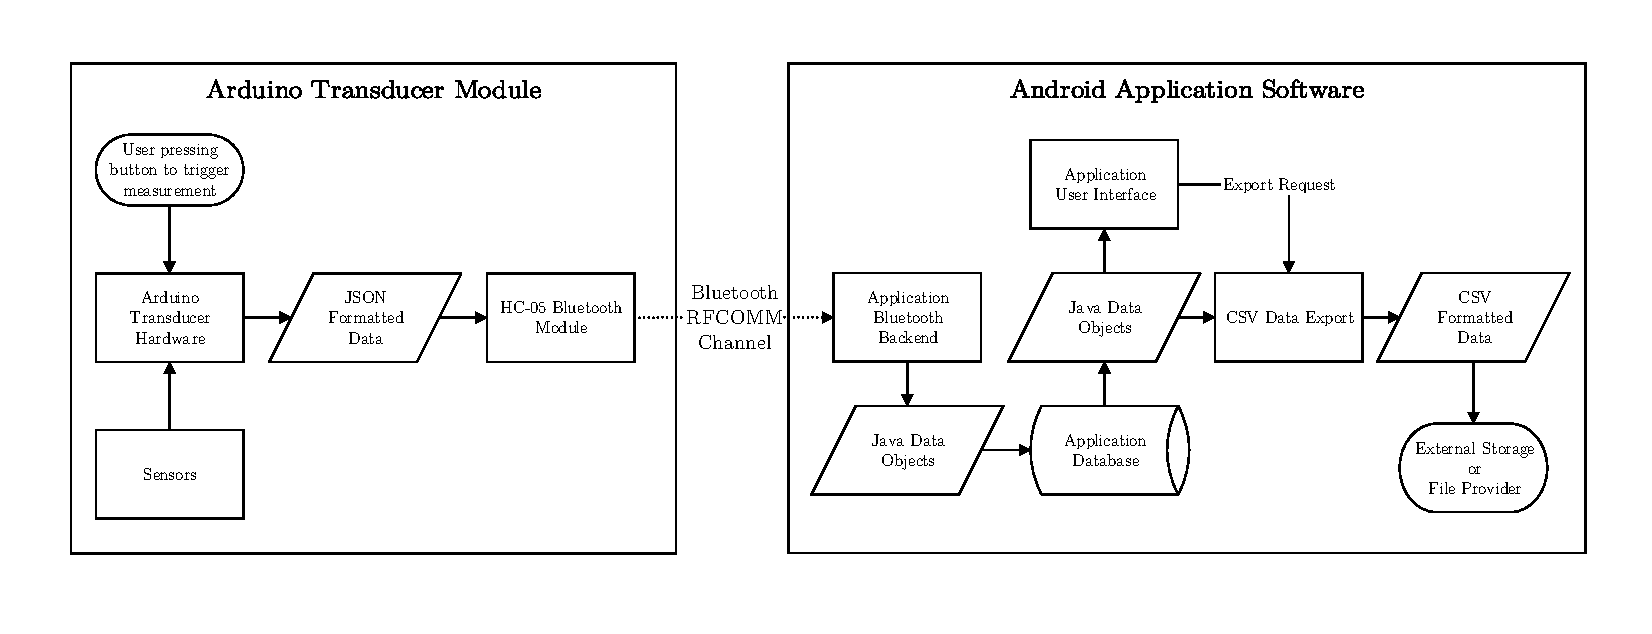
\includegraphics[width=1.1\textwidth]{src/data_flow.pdf}}
\caption{Data flow model for the overall system}
\label{fig:data_flow}
\end{figure}
\end{center}

\section{Positioning Strategies}
\label{sec:location}
Depending on the avaliable hardware and communications ressources the system shall be able to use different strategies to provide geolocalisation for the measured values. 

\subsection{Dedicated Hardware GPS Receiver}
A hardware GPS receiver can be incorporated in the sensor transducer hardware. It can operate independent of cellular network or WiFi data connections and can provide a better synchronization with the measurements triggered on the Arduino. Typically, GPS receivers are connected to the Arduino platform using a serial (TTL) connection transmitting so-called NMEA-sentences (see \cite{NMEASentences}) containing various values that can be derived from the GPS system including the location and the precise time. Dedicated hardware receivers usually allow for an external antenna to be connected which might give them a serious advantage in signal reception. The major downsides of a hardware receiver are the additional cost and the power consumption by both the GPS module and (if it is used) the external antenna.

\subsection{Android Device GPS}
Almost all Android smartphones and most Android tablets include a GPS receiver. However due to space constraints in the devices, the antennas in these devices are typically much less sensitive than dedicated external antennas. This often leads to poor GPS signal reception if the device is used in places having obstacles like trees, buildings and clouds in the signal path between the device and the GPS satellites. Compared to a hardware GPS receiver using the Android device GPS can have some advantages as most Android devices use assisted GPS to kickstart the GPS receiver with information derived from cellular and WiFi networks and some newer devices additionally include receivers for the GLONASS, BeiDou and Galileo global navigation satellite systems (GNSS).

\subsection{Googles Fused Location Provider}
The Fused Location Provider is a high-level API for localization services provided by the Google Play Services, a software library available on most Android devices (all devices using Google Play Store). The Fused Location Provider aggregates information derived from different sensors of the device and from an online service (which for example maps WiFi networks to location). The Fused Location Provider should always give results of the same or better quality compared to the device GPS at the same or a lower power consumption.

\subsection{Synchronization}
As the system might be moved during use, it is important to get not only accurate location information, but also location information synchronized to the measurements. A hardware GPS receiver does usually provide a new location in a regular interval like 1 second. This means as long as the position fix is not lost, the hardware GPS might always provide a location not older than one second. Both aforementioned Location Providers on the Android device are able to deliver location information at regular intervals too. However, using the aforementioned Location Providers in Android will lead to high energy consumption when periodic location updates are requested. As the Location Providers might also be used to provide a one-shot position fix, energy can be saved by requesting the location only in case a measured value has been received. The risk associated with this is a position drift caused by moving the device during the positioning delay. While the GPS provider can either deliver a position fix or not, the Fused Location Provider can be configured to give a high accuracy result as fast as available or give a lower accuracy result after a specified time in case a high accuracy fix is not possible. This makes the Fused Location Provider the preferred choice for one-shot location fixes.

\subsection{Performance Comparison}
With the Android platform having a huge number of different devices available, a comprehensive positioning performance test can not be undertaken in the context of this thesis. To verify the usefulness of a dedicated hardware GPS receiver however a spot test was carried out to compare the performance of some exemplary devices. The devices included in the test were the following:

\paragraph{Adafruit Ultimate GPS Breakout v3 and external Antenna}
This is a widespread dedicated hardware GPS module (see \cite{AdaGPS} for the Arduino platform. The GPS module was connected to an external antenna (see \cite{ExtAnt}) offering 28 dB of gain. The GPS module itself has a sensitivity of -165 dBm. The GPS module was equipped with a buffer battery allowing it to fix the position faster as previous knowledge of the time can be used (the module contains a real-time clock).

\paragraph{Nexus 7 (2012)}
The Nexus 7 (2012) (see \cite{Nexus7}) is a widespread Android tablet released in 2012. It does not offer a cellular data connection. For the performance comparison test, this device was set to flight mode and no data connection was available during the positioning. The data used in this test was derived using the Fused Location Provider (set to high accuracy) in one-shot mode; there was no active background GPS. The operating system used was the Android-based Resurrection Remix OS (see \cite{ResurOS}) equipped with Google Apps and the Google Play Services.

\paragraph{Ulefone Power}
The Ulefone Power (see \cite{UlePow}) is a smartphone running Android 6.0 Marshmallow. For this test, the Fused Location Provider (set to high accuracy) was used in one-shot-mode while the GPS provider was kept active in the background. An LTE cellular network connection was active at all times.

\subsubsection{Test Setup}
The test was carried out by moving the devices repeatedly between two fixed positions around 200 meters apart. The position was then recorded while all devices were at rest and at most 20 centimeters apart. Both locations have unobstructed view to the sky and the test was carried out under clear blue sky without any clouds.

\subsubsection{Test Result}
The test data has been imported into the Matlab software (see \cite{MATLAB}) and plotted to a web map. This map is shown in figure \ref{fig:gps_comparison}. While no statistical tests were carried out, performance differences can visually be deducted from the map. The raw measurement data and the script used to plot the map are included in the digital appendix.

\begin{figure*}[t]
\centering
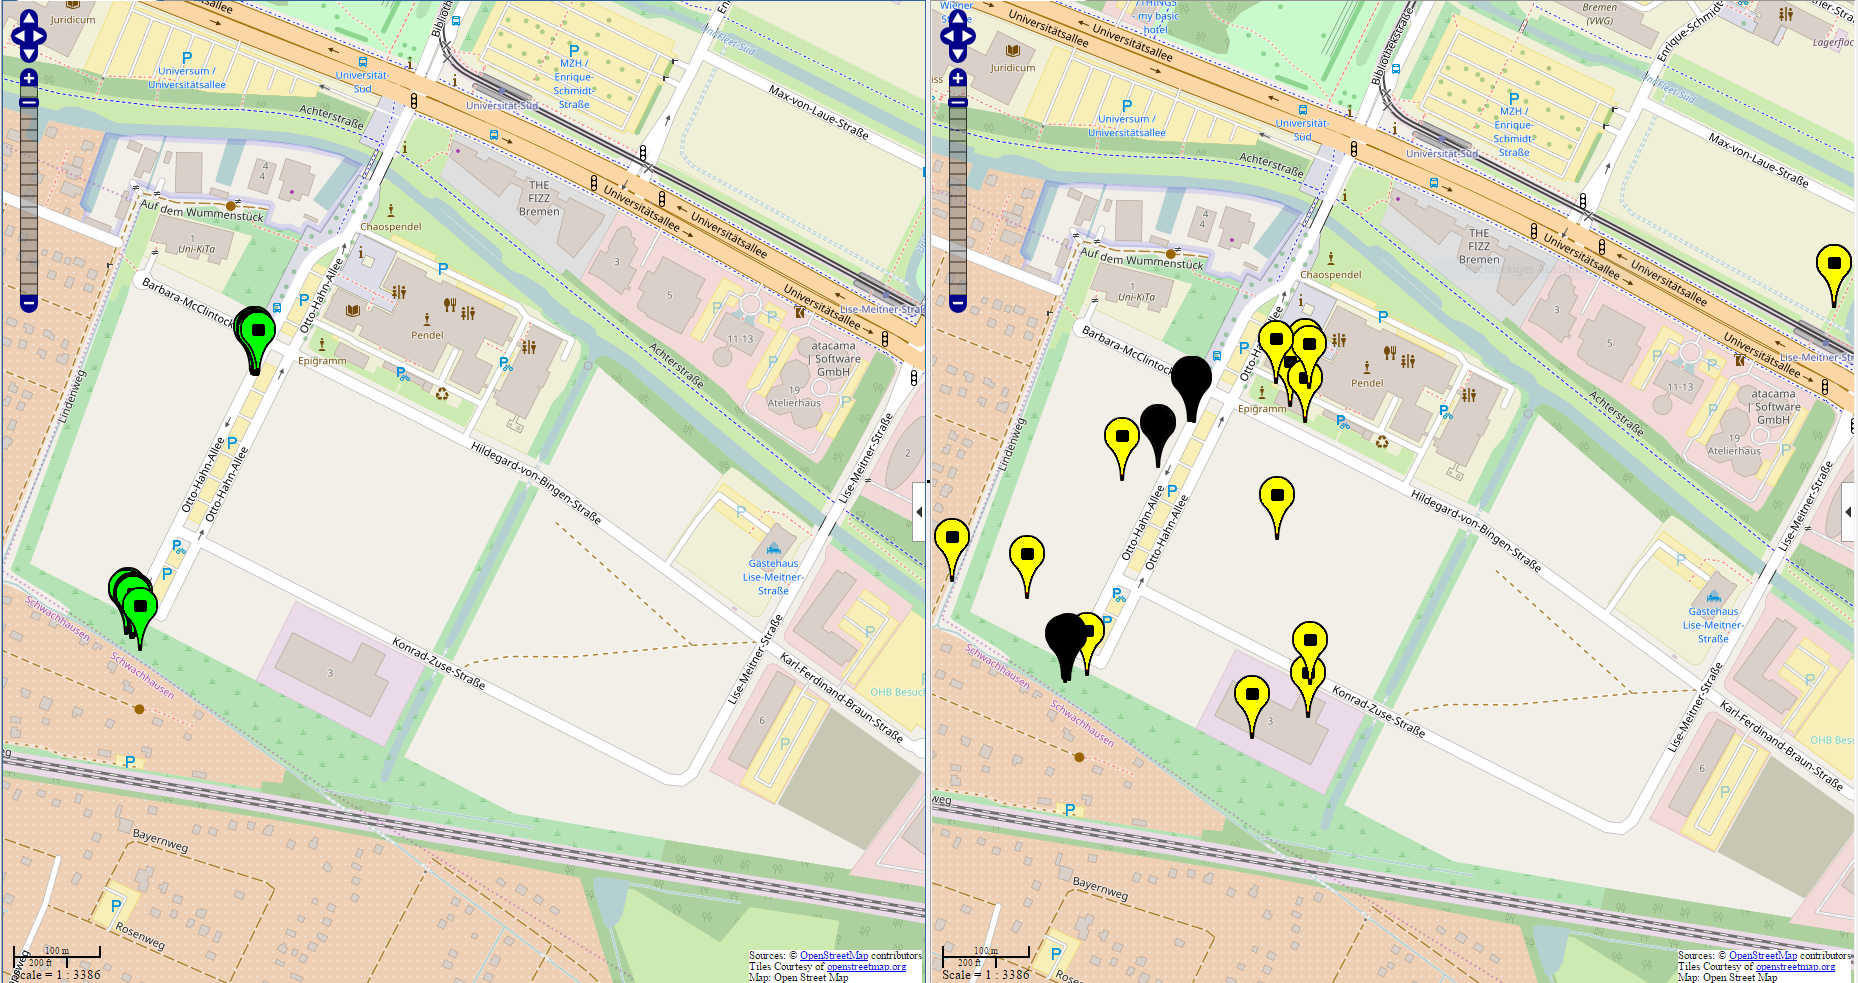
\includegraphics[width=1.0\textwidth]{src/gps_comparison.png}
\caption{Visualisation of the positioning test results. Left: Adafruit Ultimate GPS v3, Right: Black markers for the Nexus 7 and yellow markers for the Ulefone Power}
\label{fig:gps_comparison}
\end{figure*}

\subsubsection{Conclusion}
As seen on the map in figure \ref{fig:gps_comparison}, results derived from the Adafruit GPS module do vary only slightly between the measurements. The markers are covering the actual position of the measurements and do not differ by more than 10 meters from the actual position. The Nexus 7 (the black markers in the right map) exposes a similar result with one marker being on the way between the positions where the measurements have been triggered. The deviating marker marks the first measurement and is a result of movement during the positioning delay which could have been avoided if background gps positioning was enabled before this test. 

The Ulefone Power, even though its technical means to acquire a position seem much better as cellular networks and WiFi positioning were available as well, shows significant and obvious scattering of the location data acquired. The Fused Location Provider in this case reports a widely varying accuracy, but even when the reported accuracy is accounted for, the overall performance must still be considered poor compared to the other two devices.

In conclusion no general statement can be made on the positioning accuracy provided by Android devices. As a design decision, the system should therefore allow both dedicated hardware GPS receivers and the capabilities of the Android device to be used.

\subsection{Implemented Positioning Strategies}
The preferred approach is incorporating a GPS receiver in the sensor transducer hardware, however the Android app should contain means to record the location from the Android device's means of localization. 